\documentclass[10pt]{beamer}
\usetheme{SCLminimal}
\usefonttheme[onlymath]{serif}
\setbeamercovered{invisible}
\beamerdefaultoverlayspecification{<+->}

\usepackage[utf8]{inputenc}
\usepackage[english]{babel}
\usepackage[T1]{fontenc}
\usepackage{lmodern,amsmath,booktabs,setspace,mathtools,movie15}


%If you want to use section pages.
\insertsectionpages


%--------------------------------------------------------------------
%You can leave the brackets under subtitle, author and institute blank, but please retain the empty brackets.
\title[Stochastic Storm Surge Modeling using ADCIRC+SWAN\ldots]{Stochastic Storm Surge Modeling}
\subtitle{using ADCIRC+SWAN through Parallel Computing}
\singleauthor %default setting, always use on lab reports with at most 3 authors.
%\multiauthors %uncomment if true, titlepage settings for conference presentations with authors more than 3, or with multiple affiliations.
\author[JF Ray]{J Franco Ray}
\institute{
\sclaffiliation\\
\tref{jbrayo@up.edu.ph}
   }
\event{} %presentation/conference name; default (if empty): SCL Presentation
\shortevent{}%for looong conference names; it copies the event name above if empty
\date{\today}
%--------------------------------------------------------------------





\begin{document}

{\SCLtitlepagebg
\begin{frame}[plain,noframenumbering]
  \maketitle
  \insertSCLDCSUPlogos
\end{frame}}

% TOC
\begin{frame}[noframenumbering]{Outline}
\tableofcontents
\end{frame}

\section{Introduction}
\begin{frame}{Introduction}
	\begin{itemize}
		\item<1-> Typhoon Haiyan brought destructive storm surge in Tacloban City on Nov 08 2013
		\item<2-> Storm surge predictions from different agencies are not completely consistent
		\item<3-> No CFD software for stochastic storm surge
		\item<4-> We need better and more realistic model!
	\end{itemize}
\end{frame}
\begin{frame}{Research Objective}
	\begin{itemize}
		\item Tailor a model specifically for the Philippines
		\item Compute fast enough and give real-time predictions
		\item Include stochastic process in the governing equations of ADCIRC+SWAN model
		\item Investigate parameter sensitivity
	\end{itemize}
\end{frame}

\section{Related Studies}
\begin{frame}{Storm Surge Modeling}
	Can be done using deterministic models
	\begin{itemize}
		\item<1-> ADCIRC+SWAN
		\item<1-> Delft3D-FLOW+WAVE
		\item<1-> SLOSH
		\item<1-> JMA
	\end{itemize}
	Only ADCIRC+SWAN can compute in \structure{parallel}
	
	Can also use statistical analysis based from past events
\end{frame}
\begin{frame}{ADCIRC+SWAN}
	\begin{itemize}
		\item Highly developed program for solving fluid motion equations in 2D/3D
		\item Finite-element in time and finite-difference in time
		\item Uses shallow water equations and continuity equation to obtain water velocity and elevation
		\item Grid flexibility, efficiency and accuracy well documented
	\end{itemize}
\end{frame}

\section{Sensitivity Analysis}
\subsection{Wetting and Drying Algorithm}
\begin{frame}{Wetting and Drying Algorithm}{}
  \begin{itemize}
    \item<1-> If the water total depth is larger than $H_{min}$, the node remains "wet" and included in the rest of calculations.
    \item<1-> Else, the node is "dry" and removed from the calculations.
    \item<2-> If the minimum wetting velocity is larger then $U_{min}$, the node becomes "wet".
    \begin{equation*}
    U = \frac{g\left(\zeta_{i-1} - \zeta_i\right)}{\tau_i \Delta x_i}
    \end{equation*}
    \item<3-> This criterion almost becomes a height restriction if the adj node's free surface circulation is sufficiently larger than its own.
  \end{itemize}
\end{frame}

\subsection{Bottom Friction}
\begin{frame}{Bottom Friction}{}
	\begin{itemize}
		\item<1-> The parameter $\tau_0$ controls bottom friction in the model.
		\begin{equation*}
		\tau_i = \tau_0 \left(\frac{u_i}{H_i}\right)
		\end{equation*}
		\item<2-> Note that $\tau \propto \tau_0$
		\item<2-> $\tau_i$ increases in shallower, near-shore waters and directly affects the speed at which waves inundate or recede.
	\end{itemize}
\end{frame}
%%%%%%%%%%%%%%%%

\subsection{GWCE Weighing Factor}
\begin{frame}{GWCE Weighing Factor}
	\begin{itemize}
		\item<1-> The parameter $G$ is the numerical parameter that controls the balance between the wave continuity equation and the primitive continuity equation.
		\begin{equation*}
			\frac{\partial \zeta}{\partial t} + G\zeta - \nabla \cdot M = 0
		\end{equation*}
		\item<1-> As $G \rightarrow 0$: pure wave equation, $G \rightarrow \infty$: pure primitive equation.
		\item<2-> If $G$ is set too high, solution has spurious oscillations that prevent the model from capturing behavior of waves.
	\end{itemize}
\end{frame}

\section{Methodology}
\begin{frame}{Methodology}
	\begin{itemize}
		\item<1-> Disregard tweaking of $U_{min}$
		\item<2-> Adjust parameters one by one: $H_{min}, G, \tau_0$.
		\item<3-> Three dimensional analysis of parameters is \structure{very hard}.
	\end{itemize}
\end{frame}

\begin{frame}{Methodology}{observation points}
	\begin{figure}[H]
		\begin{center}
			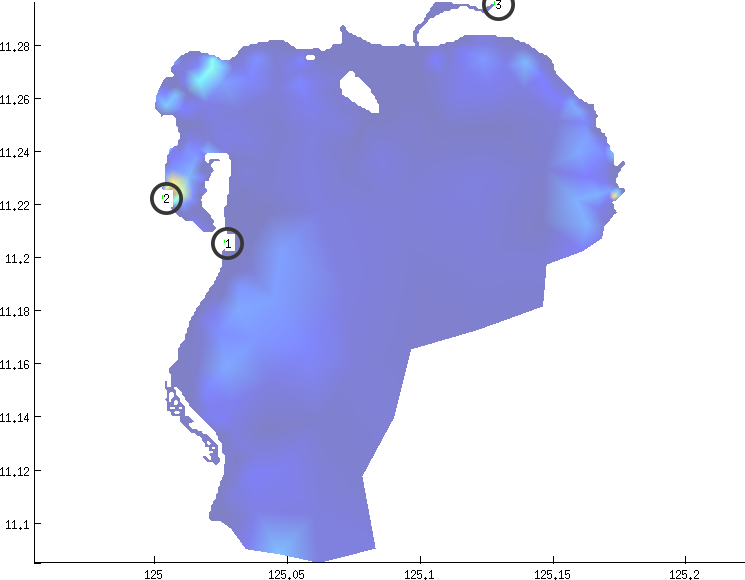
\includegraphics[width=.8\textwidth]{stations}
		\end{center}
	\end{figure}
\end{frame}

\begin{frame}{\texttt{fort.15} Input File}
	\begin{figure}[H]
		\begin{center}
			\includegraphics[width=\textwidth]{fort15}
		\end{center}
	\end{figure}
\end{frame}

\begin{frame}{Original Inputs}{$H_{min}$=0.10, $G$=0.01, $\tau_0$=0.15, $\hat{\zeta}$=5.367}
	\begin{figure}[H]
		\begin{center}
			
\includegraphics[width=\textwidth]{stoch0}
		\end{center}
	\end{figure}
\end{frame}

\section{Results}
\begin{frame}{Water Cutoff Depth}{$H_{min}$ \textbf{0.01} 0.10 0.15 0.20 0.25 0.30 0.40 0.50}
	\begin{figure}[H]
		\begin{center}
			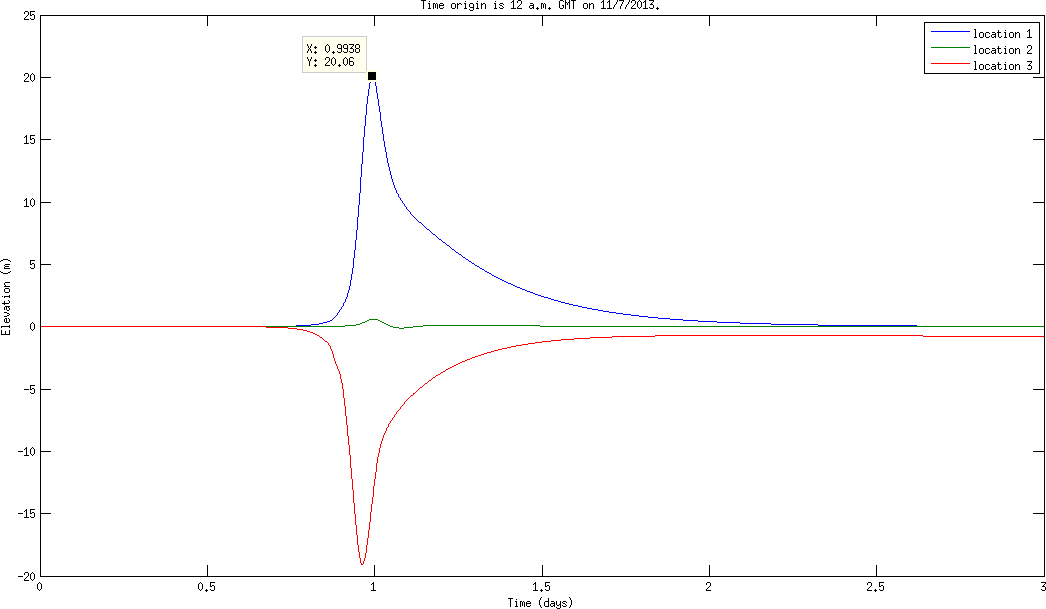
\includegraphics[width=\textwidth]{H_min/h0-01}
		\end{center}
	\end{figure}
\end{frame}

\begin{frame}{Water Cutoff Depth}{$H_{min}$ 0.01 \textbf{0.05} 0.10 0.15 0.20 0.25 0.30 0.40}
	\begin{figure}[H]
		\begin{center}
			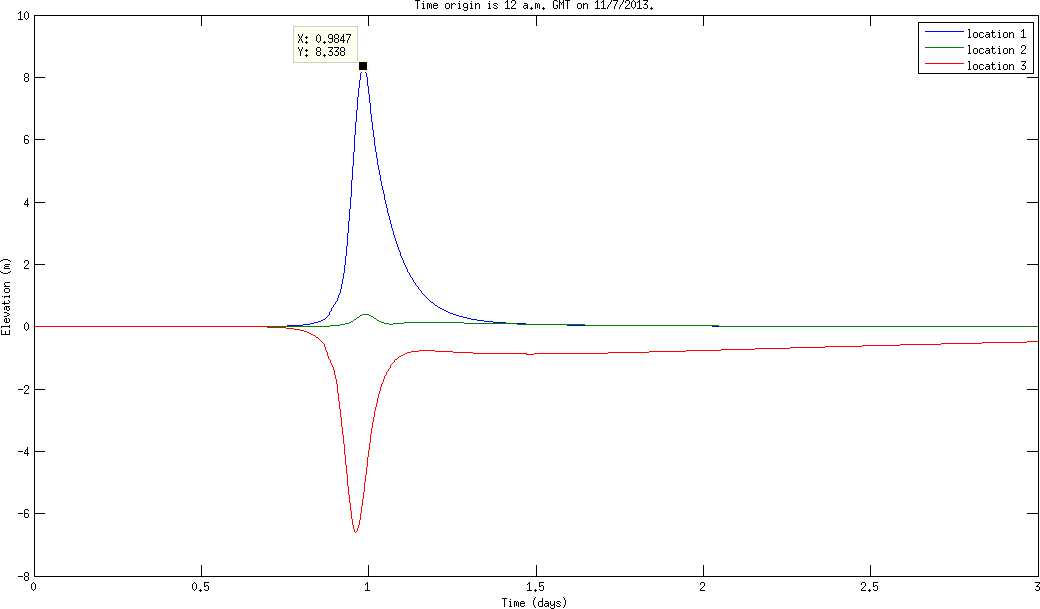
\includegraphics[width=\textwidth]{H_min/h0-05}
		\end{center}
	\end{figure}
\end{frame}

\begin{frame}{Water Cutoff Depth}{$H_{min}$ 0.01 0.05 \textbf{0.10} 0.15 0.20 0.25 0.30 0.40 0.50}
	\begin{figure}[H]
		\begin{center}
			
\includegraphics[width=\textwidth]{stoch0}
		\end{center}
	\end{figure}
\end{frame}

\begin{frame}{Water Cutoff Depth}{$H_{min}$ 0.01 0.05 0.10 \textbf{0.15} 0.20 0.25 0.30 0.40 0.50}
	\begin{figure}[H]
		\begin{center}
			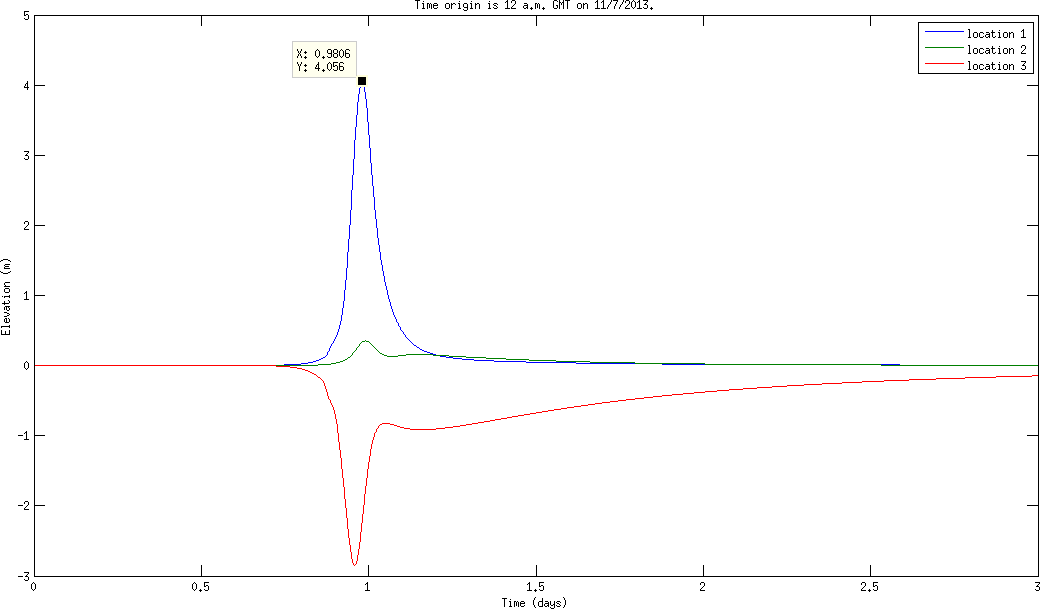
\includegraphics[width=\textwidth]{H_min/h0-15}
		\end{center}
	\end{figure}
\end{frame}

\begin{frame}{Water Cutoff Depth}{$H_{min}$ 0.01 0.05 0.10 0.15 \textbf{0.20} 0.25 0.30 0.40 0.50}
	\begin{figure}[H]
		\begin{center}
			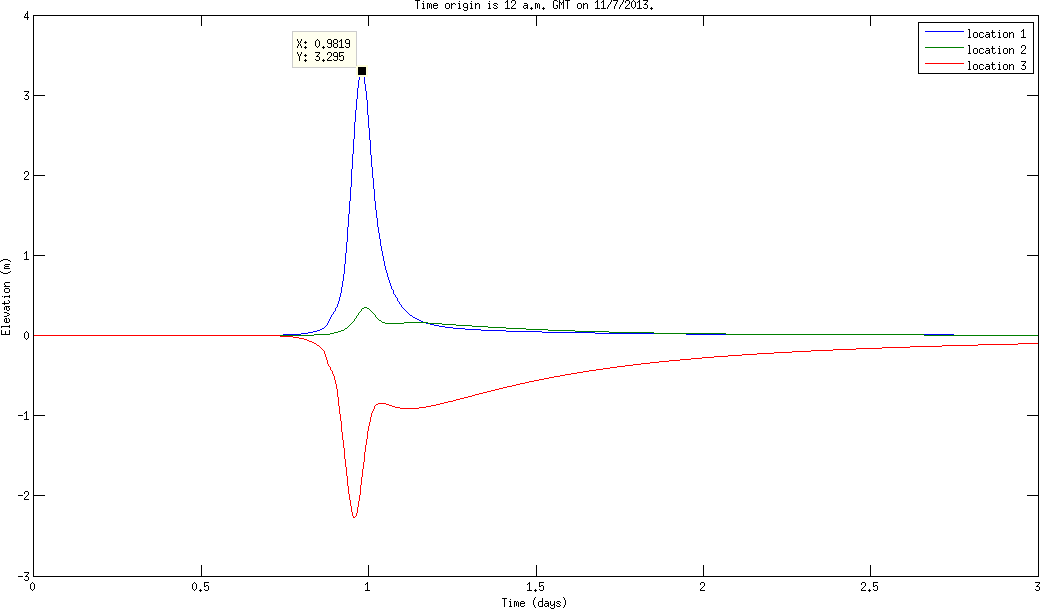
\includegraphics[width=\textwidth]{H_min/h0-2}
		\end{center}
	\end{figure}
\end{frame}

\begin{frame}{Water Cutoff Depth}{$H_{min}$ 0.01 0.05 0.10 0.15 0.20 \textbf{0.25} 0.30 0.40 0.50}
	\begin{figure}[H]
		\begin{center}
			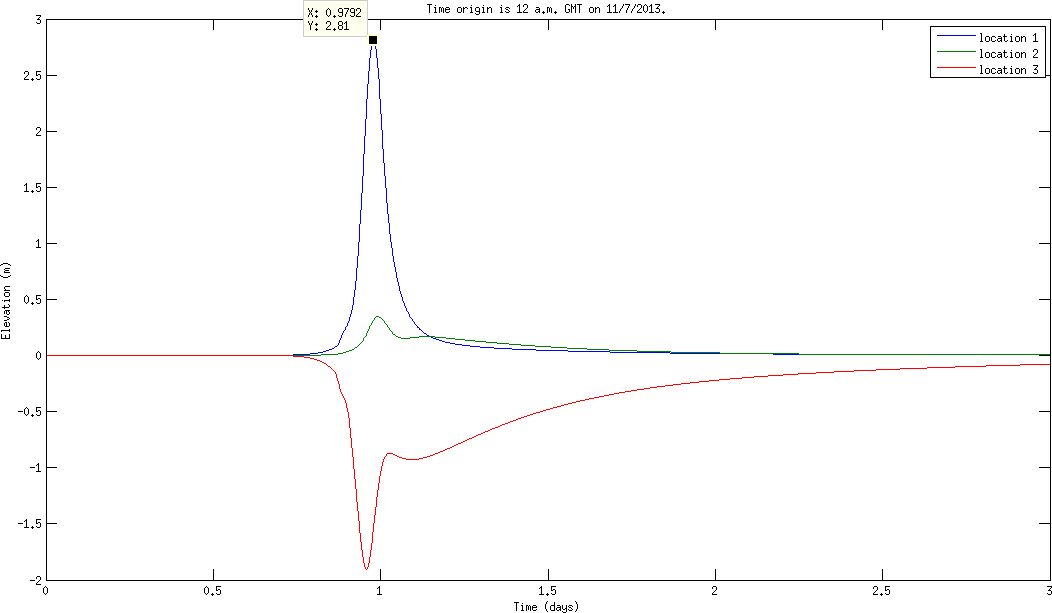
\includegraphics[width=\textwidth]{H_min/h0-25}
		\end{center}
	\end{figure}
\end{frame}

\begin{frame}{Water Cutoff Depth}{$H_{min}$ 0.01 0.05 0.10 0.15 0.20 0.25 \textbf{0.30} 0.40 0.50}
	\begin{figure}[H]
		\begin{center}
			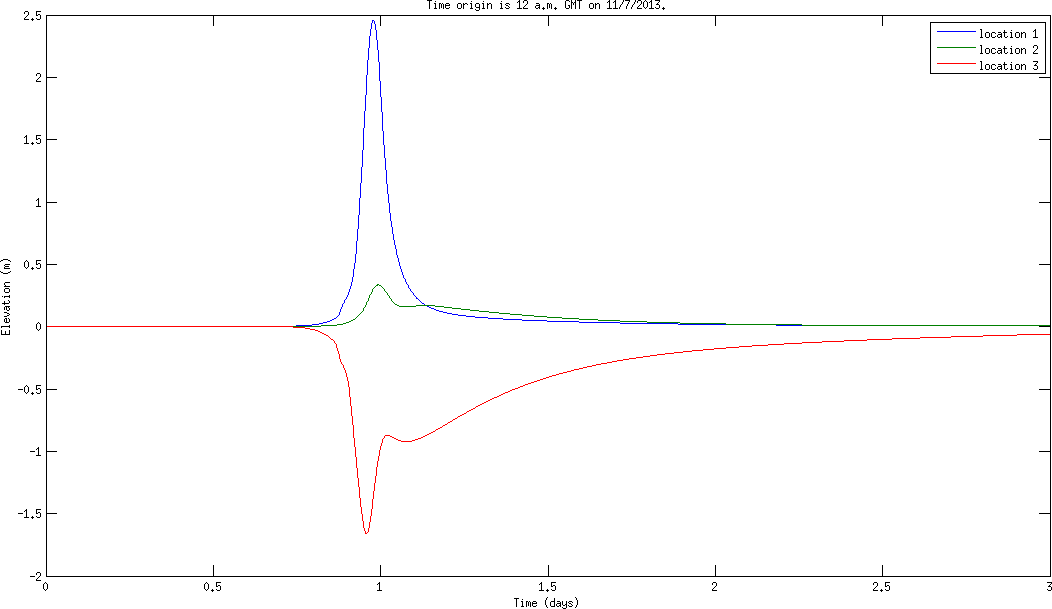
\includegraphics[width=\textwidth]{H_min/h0-3}
		\end{center}
	\end{figure}
\end{frame}

\begin{frame}{Water Cutoff Depth}{$H_{min}$ 0.01 0.05 0.10 0.15 0.20 0.25 0.30 \textbf{0.40} 0.50}
	\begin{figure}[H]
		\begin{center}
			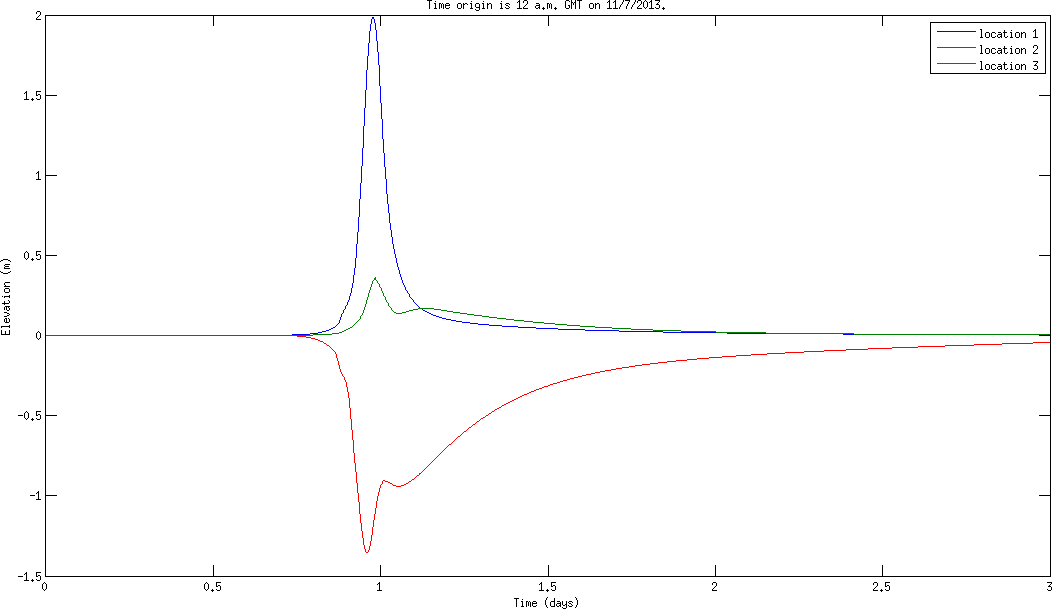
\includegraphics[width=\textwidth]{H_min/h0-4}
		\end{center}
	\end{figure}
\end{frame}

\begin{frame}{GWCE Weighing Factor}{$G$ \textbf{0.001} 0.005 0.01 0.05 0.10 0.15 0.20}
	\begin{figure}[H]
		\begin{center}
			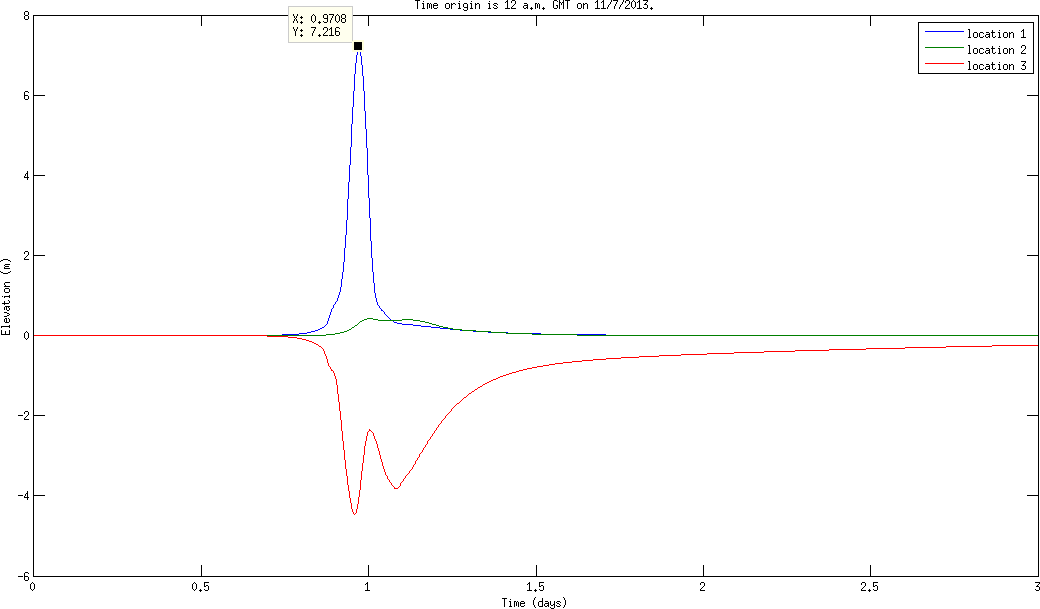
\includegraphics[width=\textwidth]{G/g0-001}
		\end{center}
	\end{figure}
\end{frame}

\begin{frame}{GWCE Weighing Factor}{$G$ 0.001 \textbf{0.005} 0.01 0.05 0.10 0.15 0.20}
	\begin{figure}[H]
		\begin{center}
			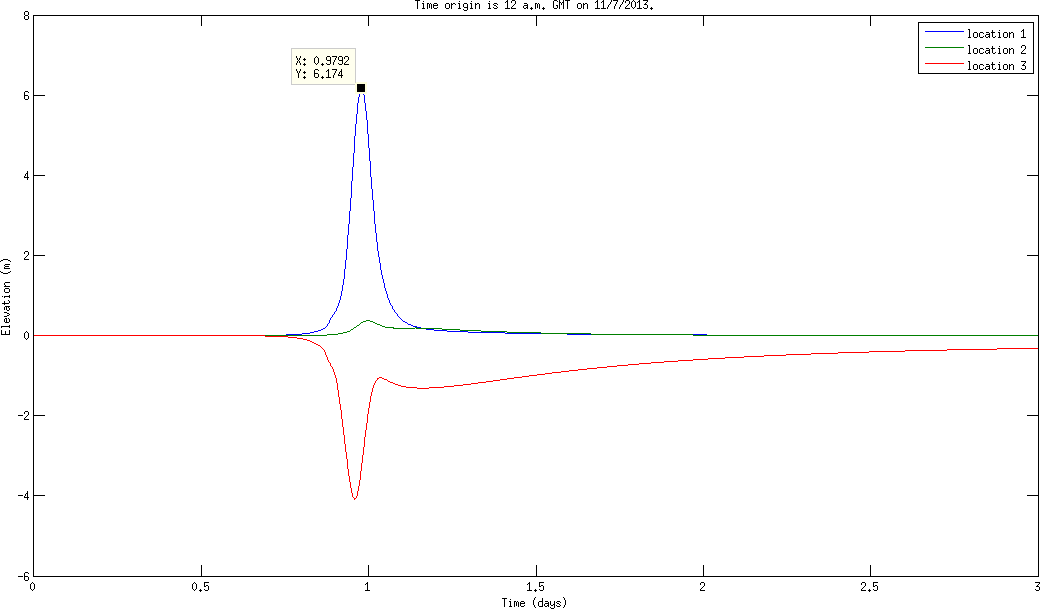
\includegraphics[width=\textwidth]{G/g0-005}
		\end{center}
	\end{figure}
\end{frame}

\begin{frame}{GWCE Weighing Factor}{$G$ 0.001 0.005 \textbf{0.01} 0.05 0.10 0.15 0.20}
	\begin{figure}[H]
		\begin{center}
			
\includegraphics[width=\textwidth]{stoch0}
		\end{center}
	\end{figure}
\end{frame}

\begin{frame}{GWCE Weighing Factor}{$G$ 0.001 0.005 0.01 0.05 0.10 \textbf{0.15} 0.20}
	\begin{figure}[H]
		\begin{center}
			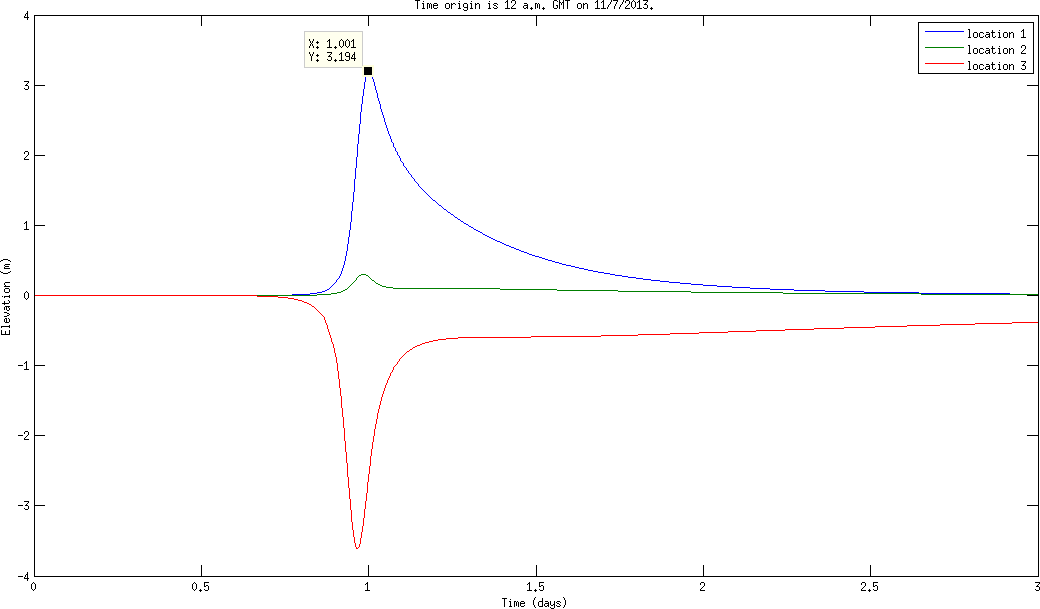
\includegraphics[width=\textwidth]{G/g0-15}
		\end{center}
	\end{figure}
\end{frame}

\begin{frame}{GWCE Weighing Factor}{$G$ 0.001 0.005 0.01 0.05 0.10 0.15 \textbf{0.20}}
	\begin{figure}[H]
		\begin{center}
			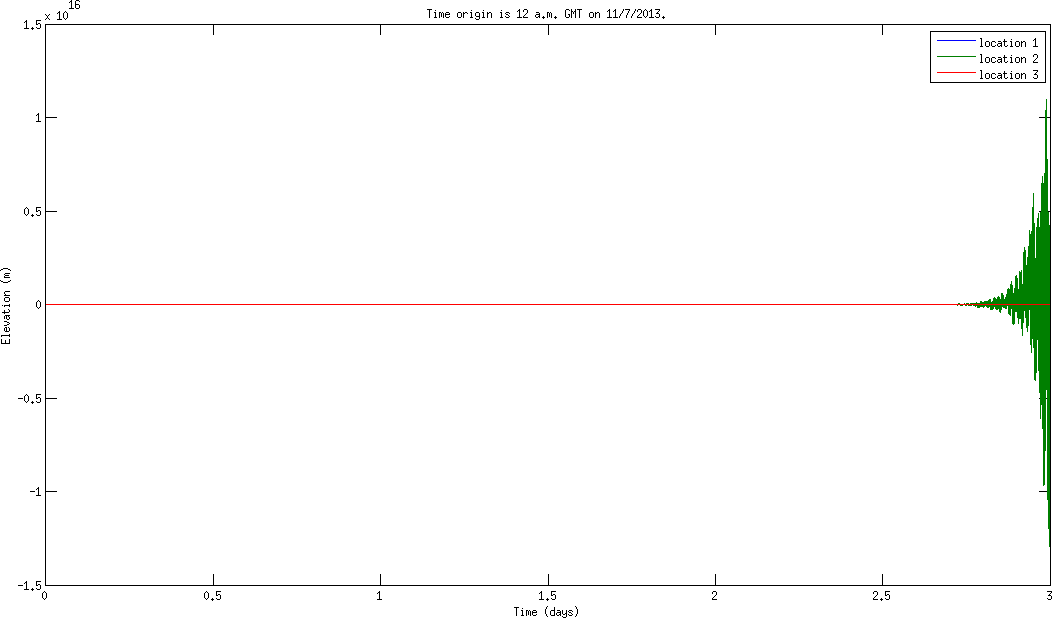
\includegraphics[width=\textwidth]{G/g0-20}
		\end{center}
	\end{figure}
\end{frame}

\begin{frame}{Bottom Friction}{$\tau_0$ \textbf{0.01} 0.05 0.10 0.15 0.20}
	\begin{figure}[H]
		\begin{center}
			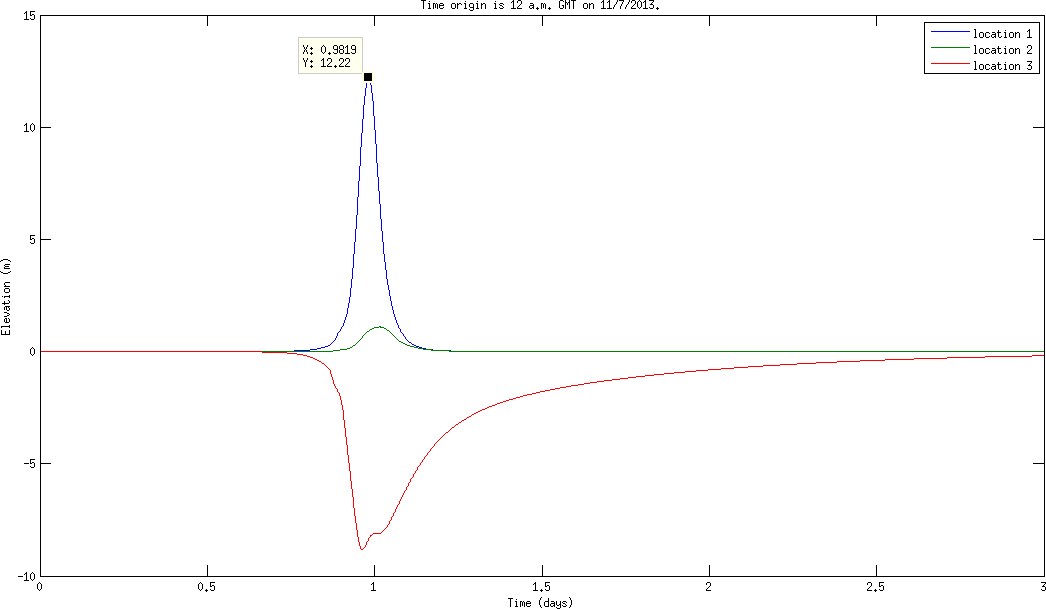
\includegraphics[width=\textwidth]{Tau/tau0-01}
		\end{center}
	\end{figure}
\end{frame}

\begin{frame}{Bottom Friction}{$\tau_0$ 0.01 \textbf{0.05} 0.10 0.15 0.20}
	\begin{figure}[H]
		\begin{center}
			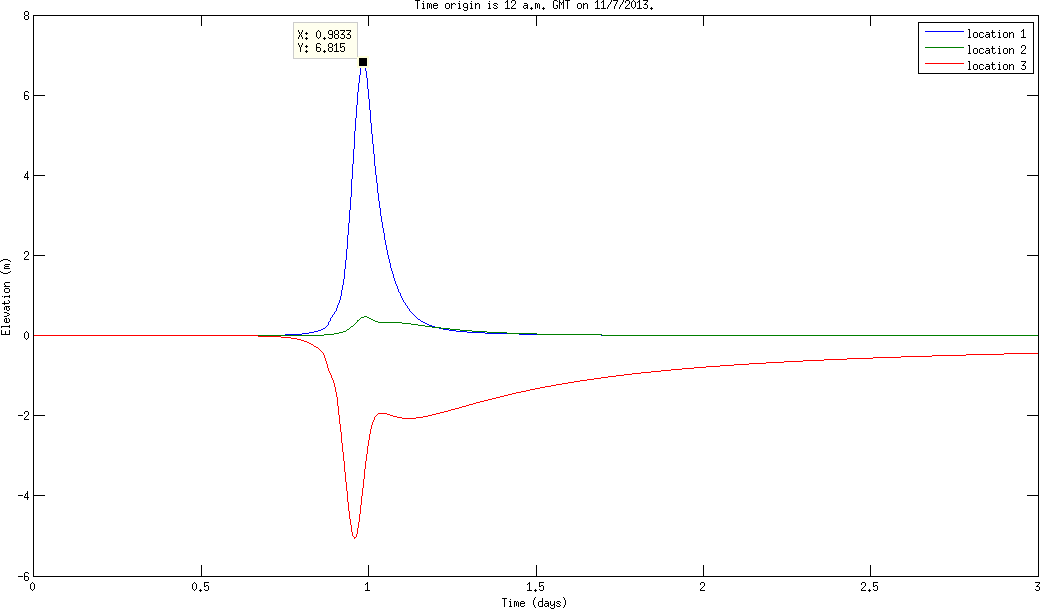
\includegraphics[width=\textwidth]{Tau/tau0-05}
		\end{center}
	\end{figure}
\end{frame}

\begin{frame}{Bottom Friction}{$\tau_0$ 0.01 0.05 \textbf{0.10} 0.15 0.20}
	\begin{figure}[H]
		\begin{center}
			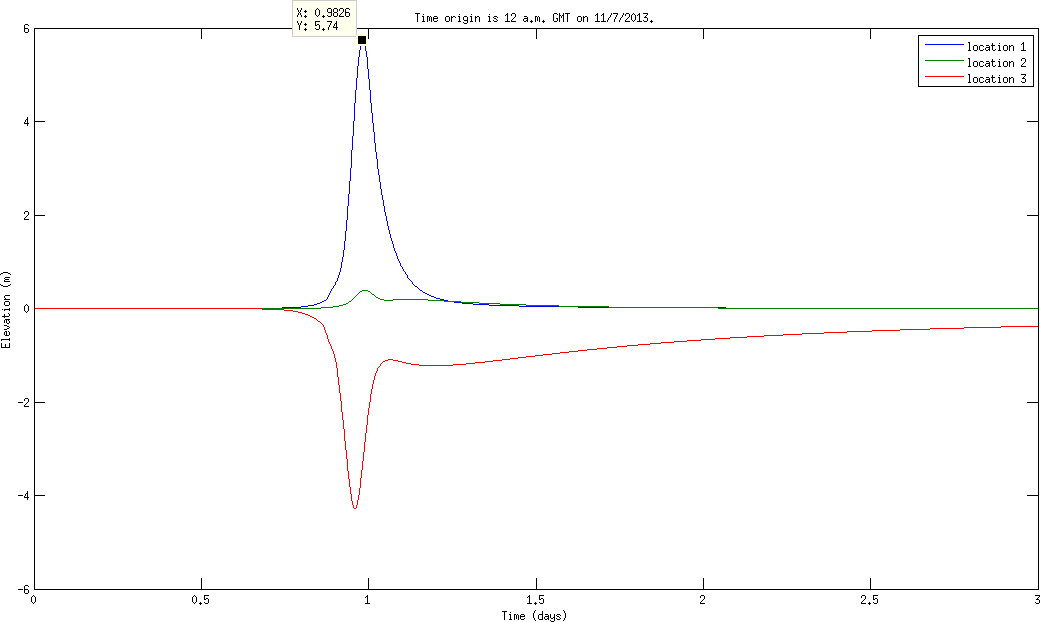
\includegraphics[width=\textwidth]{Tau/tau0-10}
		\end{center}
	\end{figure}
\end{frame}

\begin{frame}{Bottom Friction}{$\tau_0$ 0.01 0.05 0.10 \textbf{0.15} 0.20}
	\begin{figure}[H]
		\begin{center}
			
\includegraphics[width=\textwidth]{stoch0}
		\end{center}
	\end{figure}
\end{frame}

\begin{frame}{Bottom Friction}{$\tau_0$ 0.01 0.05 0.10 0.15 \textbf{0.20}}
	\begin{figure}[H]
		\begin{center}
			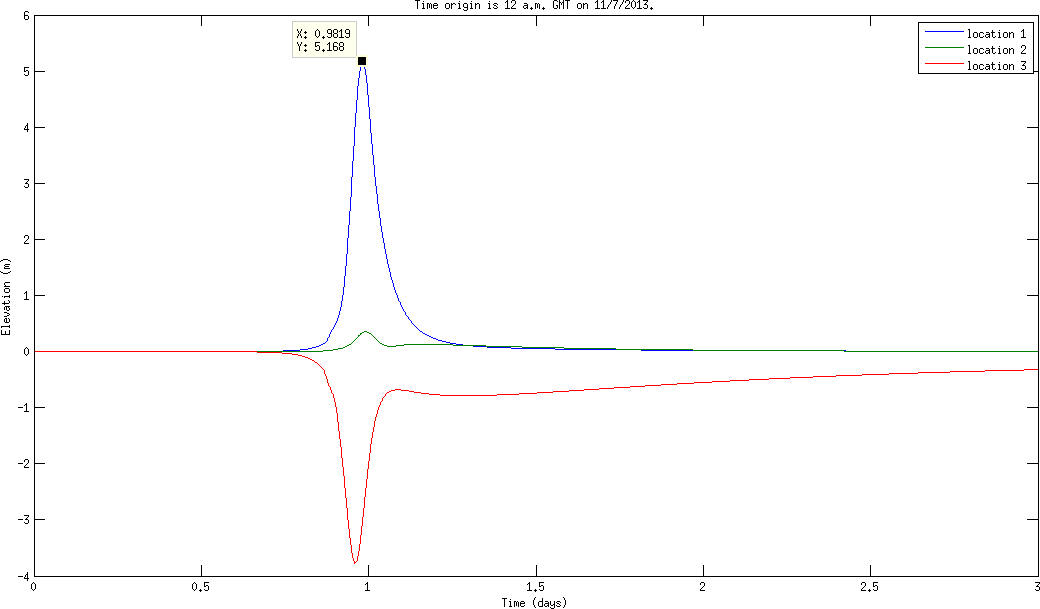
\includegraphics[width=\textwidth]{Tau/tau0-20}
		\end{center}
	\end{figure}
\end{frame}

\begin{frame}{Observations}
	\begin{itemize}
		\item<1-> Lower $H_{min}$, higher surge
		\item<1-> Higher $G$, more oscillations, unstable. Lower $G$, higher surge height; water subsides slower
		\item<1-> Lower $\tau_0$, higher surge height; water subsides slower
	\end{itemize}
\end{frame}

\begin{frame}{Conclusion}
	\begin{figure}[H]
		\includegraphics[width=\textwidth]{feat}
	\end{figure}
\end{frame}

\begin{frame}[noframenumbering]{Selected References}
\begin{thebibliography}{1}	
\bibitem<1->{stoch}
V. P. Bo\~{n}golan, et. al.
\newblock {\em Stochastic Terms in Boundary Conditions: Applications}.
\newblock Ellis College of the New York Institute of Technology., 2008.
	
\bibitem<1->{adcirc}
R. A. Luettich, Jr., et. al.
\newblock {\em ADCIRC: An Advanced Three-Dimensional Circulation Model, Theory and Methodology}.
\newblock US Army Engineer Waterways Experiment Station, Vicksburg, Mississippi, 1992.

\bibitem<1->{num}
J. C. Dietrich, et. al.
\newblock {\em Assessment of ADCIRC's Wetting and Drying Algorithm.}
\newblock Institute of Marine Sciences, University of North Carolina, 2005.
\end{thebibliography}
\end{frame}

{\SCLendpagebg
\begin{frame}[plain,noframenumbering]
\finalpage{Thank you for your attention!}
\end{frame}}




\end{document}